% !TeX root = RJwrapper.tex
\title{clarify: Simulation-Based Inference for Regression Models}


\author{by Noah Greifer, Steven Worthington, Stefano Iacus, and Gary King}

\maketitle

\abstract{%
Simulation-based inference is an alternative to the delta method for computing the uncertainty around regression post-estimation (i.e., derived) quantities such as average marginal effects, average adjusted predictions, and other functions of model parameters. It works by drawing model parameters from their joint distribution and estimating quantities of interest from each set of simulated values, which form a simulated ``posterior'' distribution of the quantity from which confidence intervals can be computed. clarify provides a simple, unified interface for performing simulation-based inference for any user-specified derived quantities as well as wrappers for common quantities of interest. clarify supports a large and growing number of models through its interface with the marginaleffects package and provides native support for multiply imputed data.
}

\hypertarget{introduction}{%
\section{Introduction}\label{introduction}}

Although regression models are frequently used in empirical research to study relationships among variables, often the quantity of substantive interest is not one of the coefficients of the model, but rather a quantity derived from the coefficients, such as predicted values or average marginal effects. Quantifying the uncertainty of these derived quantities (i.e., computing standard errors, confidence intervals, and p-values) requires additional processing. Several methods of doing so exist, including the delta method, the bootstrap, and simulation-based inference. \CRANpkg{clarify} implements simulation-based inference, which we describe below along with these other methods.

The delta method involves computing a first-order Taylor series approximation to the variance of the derived quantity, and standard Wald-based inference relies on computing quantiles based on the Normal distribution and using them to compute p-values and confidence intervals. \CRANpkg{clarify} implements an alternative to the delta method---simulation-based inference---which involves simulating a ``posterior'' distribution of the derived quantities. Simulation-based inference does not require understanding Taylor series or the calculus that underlies it, which can make it more palatable to nontechnical audiences and easier to learn for students without necessarily sacrificing statistical performance (King, Tomz, and Wittenberg 2000; Zelner 2009). Some studies have found that simulation-based inference performs as well or better than the delta method for computing derived quantities (i.e., with respect to achieving close to nominal coverage for confidence intervals), especially for complicated derived quantities and in smaller samples (MacKinnon, Lockwood, and Williams 2004; Hole 2007; Herron 1999). Its empirical performance has been particularly well studied in the context of mediation analysis, in which the quantities of interest are products and ratios of regression coefficients, where it has been shown to perform well relative to the delta method due to the non-Normality of these quantities (Tofighi and MacKinnon 2016; Preacher and Selig 2012).

The methodology \CRANpkg{clarify} relies on was developed by Krinsky and Robb (1986) and is described in King, Tomz, and Wittenberg (2000) and Herron (1999). Simulation-based inference involves taking draws from a specified joint distribution of model parameters, computing derived quantities from these draws, and collecting the derived quantities in a ``posterior'' distribution, from which uncertainty measures (standard errors and confidence intervals) can be computed. This method assumes the model parameters are drawn from a multivariate Normal (or T) distribution with means at the estimated values and covariance equal to the asymptotic covariance matrix of the estimated values, a standard assumption motivated by the central limit theorem that underlies usual inference on the original model parameters. Arriving at the posterior distribution does not require taking any derivatives or making any approximations beyond those usually used for inference on model parameter estimates, except for the approximation due to Monte Carlo error induced by sampling from a finite number of simulations (which can always be reduced by increasing the number of draws at the cost of increased computing time).

The nonparametric bootstrap is another alternative to the delta method for inference that does not require its analytic approximations (Efron and Tibshirani 1986); bootstrapping typically involves re-sampling individuals from the sample, fitting the model in each bootstrap sample, and computing the quantity of interest from each model. Although bootstrapping tends to work well in practice, especially for complex and non-Normal estimators, refitting the model repeatedly can be prohibitively time-consuming and computationally expensive, especially for complicated models or large datasets. Simulation-based inference only requires the model to be fit once, and the simulations involve taking draws from a distribution produced from the single set of estimated parameters, making it much quicker in practice and allowing the user to capitalize on the already valid estimation of the model parameters. Methods for computing valid confidence intervals in cases when the quantity of interest has a complicated distribution are better developed when bootstrapping, however (Efron and Tibshirani 1986).

More formally, we fit a regression model \(y_i = f(x_i; \beta)\), such as a linear or other generalized linear model with model coefficients \(\beta\). We assume\[
\hat{\beta} \sim \text{MVN}(\beta, \Sigma_{\hat{\beta}})
\]where \(\hat{\beta}\) is the vector of estimates of \(\beta\) and \(\Sigma_{\hat{\beta}}\) is their asymptotic covariance matrix. We define a function \(\tau(\beta)\) that represents a quantity of interest derived from the model parameters, and compute its estimate \(\widehat{\tau(\beta)}\) as \(\tau(\hat{\beta})\). To perform simulation-based inference, we take \(M\) draws \(\tilde{\beta}^{(j)}\) for \(j\in(1, \dots, M)\) from a multivariate Normal distribution with mean vector \(\mu = \hat{\beta}\) and covariance \(\Sigma = \hat{\Sigma}_{\hat{\beta}}\), where \(\hat{\Sigma}_{\hat{\beta}}\) is an estimate of the asymptotic covariance matrix of the parameter estimates. We use the distribution of \(\tilde{\tau}=\tau(\tilde{\beta})\) as the ``posterior'' distribution of \(\widehat{\tau(\beta)}\), and compute its variance as\[
\hat\sigma^2_{\widehat{\tau(\beta)}} = \frac{1}{M-1}\sum^M_{j=1}{(\tilde{\tau}^{(j)} - \bar{\tilde{\tau}})^2}
\]and quantile \(100(1-\alpha)\%\) confidence interval limits as \(\left[\tilde{\tau}_{(\frac{\alpha}{2})}, \tilde{\tau}_{(1-\frac{\alpha}{2})}\right]\) where \(\tilde{\tau}_{(q)}\) is the \(q\)th value of \(\tilde{\tau}\) when arranged in ascending order (i.e., the \(q\)th quantile of the empirical cumulative distribution function). Simulation-based Wald-type confidence intervals can be computed as \(\left[\tau(\hat{\beta}) + \hat\sigma_{\widehat{\tau(\beta)}} Z_{\frac{\alpha}{2}}, \tau(\hat{\beta}) + \hat\sigma_{\widehat{\tau(\beta)}} Z_{1-\frac{\alpha}{2}} \right]\), where \(Z_q\) is the \(q\)th quantile of a standard Normal distribution. The delta method-based Wald-type confidence intervals use this formula but with the first-order Taylor approximation to the asymptotic variance: \(\hat\sigma^2_{\widehat{\tau(\beta)}}=\nabla\tau(\hat{\beta}) \Sigma_{\hat{\beta}} \nabla\tau'(\hat{\beta})\), where \(\nabla\tau(\hat{\beta})\) is the gradient of \(\tau(\beta)\) with respect to \(\beta\) evaluated at \(\hat{\beta}\).

To compute a p-value for a hypothesis test involving the quantity of interest, i.e., \(\text{H}_0: \tau (\beta) = \tau_0\) with a given null value \(\tau_0\), we can invert the confidence interval (Thulin 2021); that is, we find the largest value of \(\alpha\) such that \(\tau_0\) is within the confidence interval and use that \(\alpha\) as the p-value for the test. For Wald-based inference (either using the simulation-based variance or delta method-based variance), this is equivalent to performing a standard two-sided Z-test using the test statistic \(Z=\left(\tau(\hat\beta)-\tau_0\right) / \hat\sigma_{\widehat{\tau(\beta)}}\). One benefit of using the quantile p-values for inference is that equivalent tests of the same hypothesis will always yield identical p-values; for example, testing the equality of two derived quantities will yield the same p-value when comparing the difference between the quantities against a null hypothesis of 0 and the ratio of the quantities against a null hypothesis of 1, as each of these hypothesis is true if and only if the other is true.

One would expect simulation-based quantile inference, simulation-based Wald inference, and delta method-based Wald inference to align when the posterior is Normally distributed around the estimate, in which case any discrepancies would be due to Monte Carlo error in the simulated values (and therefore would shrink with increasing draws). However, for low values of \(\alpha\), it may require many draws for the simulation-based intervals to stabilize; delta method-based intervals are not subject to this error. There are a few cases in which the results might diverge: in some cases, the first-order Taylor series approximation to the variance may be poor, though in practice the approximation error is small and shrinks quickly with increasing sample size. When the posterior distribution is non-Normal but symmetric around the estimate, the quantile intervals may be more accurate (i.e., in the sense of achieving closer to nominal coverage) because they do not rely on quantiles from the Normal distribution (Tofighi and MacKinnon 2016).

Another potential advantage quantile intervals can have over Wald-intervals is that when \emph{some} monotonic transformation of the estimate has a symmetric distribution centered around the transformed estimate, the quantile intervals can achieve correct coverage without requiring knowledge of \emph{which} transformation is required (Efron and Tibshirani 1986); this is true of the quantile-based p-values as well. When the distribution is not centered around the estimate and no monotonic transformation will make it so, though, neither quantile-based nor Wald-based intervals would be expected to perform well, and quantile intervals could yield even worse coverage than Wald-based intervals, a phenomenon that occurs in the context of bootstrapping {[}Efron and Tibshirani (1986){]}\footnote{We thank an anonymous reviewer for pointing out a scenario in which this could occur: for a quantity of interest with a right-skewed sampling distribution, one would prefer an estimate to the right of the quantity's true value to have a confidence interval skewed to left to capture the bulk of the sampling distribution, but in practice a quantile confidence interval would also be skewed to the right. While a symmetric Wald-based interval may not have adequate coverage, the quantile-based interval could perform even worse.}. An informal falsification test for whether such a monotonic transformation exists is whether the median of the simulated estimates is aligned with the point estimate; if it is not, there is no monotonic transformation that will yield a symmetric quantile interval with the desired coverage.

\hypertarget{related-software}{%
\section{Related Software}\label{related-software}}

Similar functionality exists in the \pkg{CLARIFY} package in Stata\footnote{Despite the similar name, the R package \CRANpkg{clarify} and the Stata package \pkg{CLARIFY} differ in several ways, one of which is that the estimates reported by \CRANpkg{clarify} in R are those computed using the original model coefficients, whereas those reported by \pkg{CLARIFY} in Stata are those computed as the average of the simulated distribution. The R implementation avoids the ``simulation-induced bias'' described by Rainey (2023).} (Tomz, Wittenberg, and King 2003) and used to be available in the \texttt{Zelig} R package (Imai, King, and Lau 2008), though there are differences in these implementations. \CRANpkg{clarify} provides additional flexibility by allowing the user to request any derived quantity, in addition to providing shortcuts for common quantities, including predictions at representative values, average marginal effects, and average dose-response functions (described below). \CRANpkg{clarify} relies on and can be seen as a companion to the \CRANpkg{marginaleffects} package (Arel-Bundock, Greifer, and Heiss Forthcoming), which offers similar functionality but primarily uses the delta method for calculating uncertainty (though simulation-based inference is supported in a more limited capacity as well).

\hypertarget{using}{%
\section{\texorpdfstring{Using \CRANpkg{clarify}}{Using }}\label{using}}

There are four steps to using \CRANpkg{clarify}:

\begin{enumerate}
\def\labelenumi{\arabic{enumi}.}
\item
  Fit the model to the data using modeling functions in supported packages.
\item
  Use \texttt{sim()} to take draws from the multivariate distribution of the estimated model coefficients.
\item
  Use \texttt{sim\_apply()} or its wrappers \texttt{sim\_setx()}, \texttt{sim\_ame()}, and \texttt{sim\_adrf()} to compute derived quantities using each simulated set of coefficients.
\item
  Use \texttt{summary()} and \texttt{plot()} to summarize and visualize the distribution of the derived quantities and perform inference on them.
\end{enumerate}

In the sections below, we will describe how to implement these steps in detail. First, we will load \CRANpkg{clarify} using \texttt{library()}.

\begin{verbatim}
library(clarify)
\end{verbatim}

For a running example, we will use the \texttt{lalonde} dataset in the \CRANpkg{MatchIt} package (Ho et al. 2011), which contains data on 614 participants enrolled in a job training program or sampled from a survey (Dehejia and Wahba 1999). The treatment variable is \texttt{treat} and the outcome is \texttt{re78}, and all other variables are confounders. Although the original use of this dataset was to estimate the effect of \texttt{treat} on \texttt{re78}, we will use it more generally to demonstrate all of \CRANpkg{clarify}'s capabilities. In addition, we will use a transformation of the outcome variable to demonstrate applications to nonlinear models, for which the benefits of simulation-based inference are more apparent.

\begin{verbatim}
data("lalonde", package = "MatchIt")

# Create a binary outcome variable
lalonde$re78_0 <- ifelse(lalonde$re78 > 0, 1, 0)

head(lalonde)
\end{verbatim}

\begin{verbatim}
#>      treat age educ   race married nodegree re74 re75       re78 re78_0
#> NSW1     1  37   11  black       1        1    0    0  9930.0460      1
#> NSW2     1  22    9 hispan       0        1    0    0  3595.8940      1
#> NSW3     1  30   12  black       0        0    0    0 24909.4500      1
#> NSW4     1  27   11  black       0        1    0    0  7506.1460      1
#> NSW5     1  33    8  black       0        1    0    0   289.7899      1
#> NSW6     1  22    9  black       0        1    0    0  4056.4940      1
\end{verbatim}

\hypertarget{fitting-the-model}{%
\subsection{1. Fitting the model}\label{fitting-the-model}}

The first step is to fit the model. \CRANpkg{clarify} can operate on a large set of models (those supported by \CRANpkg{marginaleffects}), including generalized linear models, multinomial models, multivariate models, and instrumental variable models, many of which are available in other R packages. Even if \CRANpkg{clarify} does not offer direct support for a given model, there are ways to use its functionality regardless (explained in more detail below).

Because we are computing derived quantities, it is not critical to parameterize the model in such a way that the coefficients are interpretable, e.g., by using a model with interpretable coefficients or centering predictors. Below, we will fit a probit regression model for the outcome given the treatment and confounders. Coefficients in probit regression do not have a straightforward interpretation, but that does not matter; our quantities of interest can be expressed as derived quantities---functions of the model parameters, such as predictions, counterfactual predictions, and averages and contrasts of them.

\begin{verbatim}
fit <- glm(re78_0 ~ treat * married + age + educ + race +
             nodegree + re74 + re75, data = lalonde,
           family = binomial("probit"))
\end{verbatim}

\hypertarget{drawing-from-the-coefficient-distribution}{%
\subsection{2. Drawing from the coefficient distribution}\label{drawing-from-the-coefficient-distribution}}

After fitting the model, we will use \texttt{sim()} to draw coefficients from their sampling distribution. The sampling distribution is assumed to be multivariate Normal or multivariate T with appropriate degrees of freedom, with a mean vector equal to the estimated coefficients and a covariance matrix equal to the asymptotic covariance matrix extracted from the model. The arguments to \texttt{sim()} are listed below:

\begin{verbatim}
sim(fit = , n = , vcov = , coefs = , dist = )
\end{verbatim}

\begin{itemize}
\item
  \texttt{fit} -- the fitted model object, the output of the call to the fitting function (e.g., \texttt{glm()})
\item
  \texttt{n} -- the number of simulated values to draw; by default, 1000. More values will yield more replicable and precise results at the cost of speed.
\item
  \texttt{vcov} -- either the covariance matrix of the estimated coefficients, a function used to extract it from the model (e.g., \texttt{sandwich::vcovHC()} for the robust covariance matrix), or a string or formula giving a code for extracting the covariance matrix, which is passed to \texttt{marginaleffects::get\_vcov()}. If left unspecified, the default covariance matrix will be extracted from the model.
\item
  \texttt{coefs} -- either a vector of coefficients to be sampled or a function to extract them from the fitted model. If left unspecified, the default coefficients will be extracted from the model. Typically this does not need to be specified.
\item
  \texttt{dist} -- the name of the distribution from which to draw the sampled coefficients. Can be \texttt{"normal"} for a Normal distribution or \texttt{t(\#)} for a T-distribution, where \texttt{\#} represents the degrees of freedom. If left unspecified, \texttt{sim()} will decide on which distribution makes sense given the characteristics of the model (the decision is made by \texttt{insight::get\_df()} with \texttt{type\ =\ "wald"}). Typically this does not need to be specified.
\end{itemize}

If one's model is not supported by \CRANpkg{clarify}, one can omit the \texttt{fit} argument and just specify the \texttt{vcov} and \texttt{coefs} argument, which will draw the coefficients from the distribution named in \texttt{dist} (\texttt{"normal"} by default).

\texttt{sim()} uses a random number generator to draw the sampled coefficients from the sampling distribution, so a seed should be set using \texttt{set.seed()} to ensure results are replicable across sessions. Using more iterations (i.e., increasing \texttt{n}) yields results that will be more stable across runs even when a seed is not set.

The output of the call to \texttt{sim()} is a \texttt{clarify\_sim} object, which contains the sampled coefficients, the original model fit object if supplied, and the coefficients and covariance matrix used to sample.

\begin{verbatim}
set.seed(1234)

# Drawing 1000 simulated coefficients using an HC2 robust
# covariance matrix
s <- sim(fit, n = 1000,
         vcov = "HC2")

s
\end{verbatim}

\begin{verbatim}
#> A `clarify_sim` object
#>  - 11 coefficients, 1000 simulated values
#>  - sampled distribution: multivariate normal
#>  - original fitting function call:
#> 
#> glm(formula = re78_0 ~ treat * married + age + educ + race + 
#>     nodegree + re74 + re75, family = binomial("probit"), data = lalonde)
\end{verbatim}

\hypertarget{computing-derived-quantities}{%
\subsection{3. Computing derived quantities}\label{computing-derived-quantities}}

After sampling the coefficients, one can compute derived quantities on each set of sampled coefficients and store the result, which represents the ``posterior'' distribution of the derived quantity, as well as on the original coefficients, which are used as the final estimates. The core functionality is provided by \texttt{sim\_apply()}, which accepts a \texttt{clarify\_sim} object from \texttt{sim()} and a function to compute and return one or more derived quantities, then applies that function to each set of simulated coefficients. The arguments to \texttt{sim\_apply()} are below:

\begin{verbatim}
sim_apply(sim = , FUN = , verbose = , cl = , ...)
\end{verbatim}

\begin{itemize}
\item
  \texttt{sim} -- a \texttt{clarify\_sim} object; the output of a call to \texttt{sim()}.
\item
  \texttt{FUN} -- a function that takes in either a model fit object or a vector of coefficients and returns one or more derived quantities. The first argument should be named \texttt{fit} to take in a model fit object or \texttt{coefs} to take in coefficients.
\item
  \texttt{verbose} -- whether to display a progress bar.
\item
  \texttt{cl} -- an argument that controls parallel processing, which can be the number of cores to use or a cluster object resulting from \texttt{parallel::makeCluster()}.
\item
  \texttt{...} -- further arguments to \texttt{FUN}.
\end{itemize}

The \texttt{FUN} argument can be specified in one of two ways: either as a function that takes in a model fit object (e.g., a \texttt{glm} or \texttt{lm} object, the output of a call to \texttt{glm()} or \texttt{lm()}) or a function that takes in a vector of coefficients. The latter will always work but the former only works for supported models. When the function takes in a model fit object, \texttt{sim\_apply()} will first insert each set of sampled coefficients into the model fit object and then supply the modified model to \texttt{FUN}.

For example, we will let our derived quantity of interest be the predicted probability of the outcome for participant PSID1. We specify our \texttt{FUN} function as follows:

\begin{verbatim}
sim_fun1 <- function(fit) {
  predict(fit, newdata = lalonde["PSID1",], type = "response")
}
\end{verbatim}

The \texttt{fit} object supplied to this function will be one in which the coefficients have been set to their values in a draw from their sampling distribution as generated by \texttt{sim()}. We then supply the function to \texttt{sim\_apply()} to simulate the sampling distribution of the predicted value of interest:

\begin{verbatim}
est1 <- sim_apply(s, FUN = sim_fun1, verbose = FALSE)

est1
\end{verbatim}

\begin{verbatim}
#> A `clarify_est` object (from `sim_apply()`)
#>  - 1000 simulated values
#>  - 1 quantity estimated:                
#>  PSID1 0.9757211
\end{verbatim}

The resulting \texttt{clarify\_est} object contains the simulated estimates in matrix form as well as the estimate computed on the original coefficients. We will examine the posterior distribution shortly, but first we will demonstrate computing a derived quantity from the coefficients directly.

The \texttt{race} variable is a factor, and the \texttt{black} category is used as the reference level, so it is not immediately clear whether there is a difference between the coefficients \texttt{racehispan} and \texttt{racewhite}, which represent the non-reference categories \texttt{hispan} and \texttt{white}. To compare these two directly, we can use \texttt{sim\_apply()} to compute a derived quantity that corresponds to the difference between them.

\begin{verbatim}
sim_fun2 <- function(coefs) {
  hispan <- unname(coefs["racehispan"])
  white <- unname(coefs["racewhite"])
  
  c("w - h" = white - hispan)
}

est2 <- sim_apply(s, FUN = sim_fun2, verbose = FALSE)

est2
\end{verbatim}

\begin{verbatim}
#> A `clarify_est` object (from `sim_apply()`)
#>  - 1000 simulated values
#>  - 1 quantity estimated:                  
#>  w - h -0.09955915
\end{verbatim}

The function supplied to \texttt{FUN} can be arbitrarily complicated and return as many derived quantities as one wants, though the slower each run of \texttt{FUN} is, the longer it will take to simulate the derived quantities. Using parallel processing by supplying an argument to \texttt{cl} can sometimes dramatically speed up evaluation.

There are several functions in \CRANpkg{clarify} that serve as convenience wrappers for \texttt{sim\_apply()} to automate some common derived quantities of interest. These include

\begin{itemize}
\item
  \texttt{sim\_setx()} -- computing predicted values and first differences at representative or user-specified values of the predictors
\item
  \texttt{sim\_ame()} -- computing average adjusted predictions, contrasts of average adjusted predictions, and average marginal effects
\item
  \texttt{sim\_adrf()} -- computing average dose-response functions and average marginal effects functions
\end{itemize}

These are described in their own sections below. In addition, there are functions that have methods for \texttt{clarify\_est} objects, including \texttt{cbind()} for combining two \texttt{clarify\_est} objects together and \texttt{transform()} for computing quantities that are derived from the already-computed derived quantities. These are also described in their own sections below.

\hypertarget{summarize-and-visualize-the-simulated-distribution}{%
\subsection{4. Summarize and visualize the simulated distribution}\label{summarize-and-visualize-the-simulated-distribution}}

To examine the uncertainty around and perform inference on our estimated quantities, we can use \texttt{plot()} and \texttt{summary()} on the \texttt{clarify\_est} object.

\texttt{plot()} displays a density plot of the resulting estimates across the simulations, with markers identifying the point estimate (computed using the original model coefficients as recommended by Rainey (2023)) and, optionally, uncertainty bounds (which function like confidence or credible interval bounds). The arguments to \texttt{plot()} are below:

\begin{verbatim}
plot(x = , parm = , ci = , level = , method = , reference =)
\end{verbatim}

\begin{itemize}
\item
  \texttt{x} -- the \texttt{clarify\_est} object (the output of a call to \texttt{sim\_apply()}).
\item
  \texttt{parm} -- the names or indices of the quantities to be plotted if more than one was estimated in \texttt{sim\_apply()}; if unspecified, all will be plotted.
\item
  \texttt{ci} -- whether to display lines at the uncertainty bounds. The default is \texttt{TRUE} to display them.
\item
  \texttt{level} -- if \texttt{ci} is \texttt{TRUE}, the desired two-sided confidence level. The default is .95 so that that the bounds are at the .025 and .975 quantiles when \texttt{method} (see below) is \texttt{"quantile"}.
\item
  \texttt{method} -- if \texttt{ci} is \texttt{TRUE}, the method used to compute the bounds. Allowable methods include thea Normal approximation (\texttt{"wald"}) or using the quantiles of the resulting distribution (\texttt{"quantile"}). The Normal approximation involves multiplying the standard deviation of the estimates (i.e., which functions like the standard error of the sampling distribution) by the critical Z-statistic computed using \texttt{(1-level)/2} to create a symmetric margin of error around the point estimate. The default is \texttt{"quantile"} to instead use quantile-based bounds.
\item
  \texttt{reference} -- whether to display a normal density over the plot for each estimate and an indicator line for the median of the estimate. The default is \texttt{FALSE} to omit them.
\end{itemize}

Below, we plot the first estimate we computed above, the predicted probability for participant PSID1:

\begin{verbatim}
plot(est1, reference = TRUE, ci = FALSE)
\end{verbatim}

\begin{center}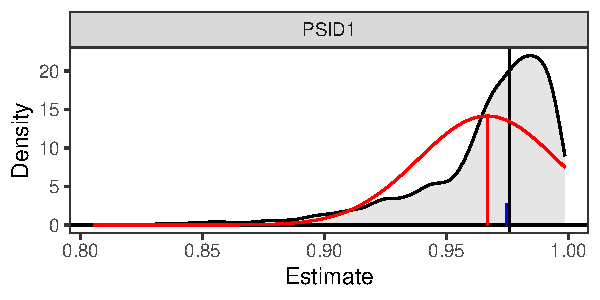
\includegraphics{figures/plot1-1} \end{center}

Overlaid on the plot in red is a Normal distribution with the same mean and standard deviation as the simulated values; this is requested by setting \texttt{reference\ =\ TRUE}. From the plot, one can see that the distribution of simulated values is non-Normal, asymmetrical, and not centered around the estimate, with no values falling above 1 because the outcome is a predicted probability. Given its non-Normality, the quantile-based bounds may be more appropriate than those resulting from the Normal approximation, as the bounds computed from the Normal approximation would be outside the bounds of the estimate. The blue reference line for the median of the estimates is close to the point estimate, suggesting it is possible for a monotonic transformation to have a symmetric distribution around the estimate\footnote{In fact, we know the inverse link function for the model (i.e., the Normal distribution function \texttt{qnorm()}) is such a transformation in this case; \CRANpkg{marginaleffects} and other packages that implement the delta method for confidence intervals around model predictions typically automatically compute confidence intervals on the transformed predictions before transforming the intervals back using the model's link function. As long as such a transformation exists, the quantile intervals will be as valid as those that rely on transforming and back-transforming.}. The plot itself is a \texttt{ggplot} object that can be modified using \texttt{ggplot2} syntax.

We can use \texttt{summary()} to display the value of the point estimate, the uncertainty bounds, and other statistics that describe the distribution of estimates. The arguments to \texttt{summary()} are below:

\begin{verbatim}
summary(object = , parm = , level = , method = , null = )
\end{verbatim}

\begin{itemize}
\item
  \texttt{object} -- the \texttt{clarify\_est} object (the output of a call to \texttt{sim\_apply()}).
\item
  \texttt{parm} -- the names or indices of the quantities to be displayed if more than one was estimated in \texttt{sim\_apply()}; if unspecified, all will be displayed.
\item
  \texttt{level} -- the desired two-sided confidence level. The default is .95 so that that the bounds are at the .025 and .975 quantiles when method (see below) is \texttt{"quantile"}.
\item
  \texttt{method} -- the method used to compute the uncertainty bounds. Allowable methods include a Normal approximation (\texttt{"wald"}) or using the quantiles of the resulting distribution (\texttt{"quantile"}). See \texttt{plot()} above.
\item
  \texttt{null} -- an optional argument specifying the desired null value in a hypothesis test for the estimates. If specified, a p-value will be computed using either a standard Z-test (if \texttt{method} is \texttt{"wald"}) or an inversion of the uncertainty interval (described below). The default is not to display any p-values.
\end{itemize}

We can use \texttt{summary()} with the default arguments on our first \texttt{clarify\_est} object to view the point estimate and quantile-based uncertainty bounds.

\begin{verbatim}
summary(est1)
\end{verbatim}

\begin{verbatim}
#>       Estimate 2.5 % 97.5 %
#> PSID1    0.976 0.890  0.996
\end{verbatim}

Our second estimated quantity, the difference between two regression coefficients, is closer to Normally distributed, as the plot below demonstrates (and would be expected theoretically), so we will use the Normal approximation to test the hypothesis that difference differs from 0.

\begin{verbatim}
plot(est2, reference = TRUE, ci = FALSE)
\end{verbatim}

\begin{center}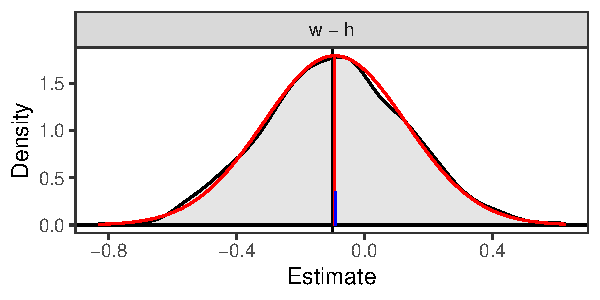
\includegraphics{figures/plot2-1} \end{center}

\begin{verbatim}
summary(est2, method = "wald", null = 0)
\end{verbatim}

\begin{verbatim}
#>       Estimate   2.5 %  97.5 % Std. Error Z value P-value
#> w - h  -0.0996 -0.5352  0.3361     0.2223   -0.45    0.65
\end{verbatim}

The uncertainty intervals and p-values in the \texttt{summary()} output are computed using the Normal approximation because we set \texttt{method\ =\ "wald"}, and the p-value for the test that our estimate is equal to 0 is returned because we set \texttt{null\ =\ 0}. Note that the Normal approximation should be used only when the simulated posterior distribution is both close to Normal and centered around the estimate (i.e., when the mean of the simulated values {[}red vertical line{]} coincides with the estimate computed on the original coefficients {[}black vertical line{]}). In such cases, however, the delta method will likely perform as well, if not better, and all of its other benefits apply (i.e., it is computationally quicker and not subject to Monte Carlo error).

\hypertarget{sim_apply-wrappers-sim_setx-sim_ame-sim_adrf}{%
\section{\texorpdfstring{\texttt{sim\_apply()} Wrappers: \texttt{sim\_setx()}, \texttt{sim\_ame()}, \texttt{sim\_adrf()}}{sim\_apply() Wrappers: sim\_setx(), sim\_ame(), sim\_adrf()}}\label{sim_apply-wrappers-sim_setx-sim_ame-sim_adrf}}

\texttt{sim\_apply()} can be used to compute the simulated posterior distribution for an arbitrary derived quantity of interest, but there are some quantities that are common in applied research and may otherwise be somewhat challenging to program by hand, so \CRANpkg{clarify} provides shortcut functions to make computing these quantities simple. These functions include \texttt{sim\_setx()}, \texttt{sim\_ame()}, and \texttt{sim\_adrf()}. Each of these can be used only when regression models compatible with \CRANpkg{clarify} are supplied to the original call to \texttt{sim()}.

Like \texttt{sim\_apply()}, each of these functions is named \texttt{sim\_*()}, which signifies that they are to be used on an object produced by \texttt{sim()} (i.e., a \texttt{clarify\_sim} object). (Multiple calls to these functions can be applied to the same \texttt{clarify\_sim} object and combined; see the \texttt{cbind()} section below.) These functions are described below.

\hypertarget{sim_setx-predictions-at-representative-values}{%
\subsection{\texorpdfstring{\texttt{sim\_setx()}: predictions at representative values}{sim\_setx(): predictions at representative values}}\label{sim_setx-predictions-at-representative-values}}

\texttt{sim\_setx()} provides an interface to compute predictions at representative and user-supplied values of the predictors. For example, we might want to know what the effect of treatment is for a ``typical'' individual, which corresponds to the contrast between two model-based predictions (i.e., one under treatment and one under control for a unit with ``typical'' covariate values). This functionality mirrors the \texttt{setx()} and \texttt{setx1()} functionality of \texttt{Zelig} (which is where its name originates) and provides similar functionality to functions in \CRANpkg{modelbased}, \CRANpkg{emmeans}, \CRANpkg{effects}, and \CRANpkg{ggeffects}.

For each predictor, the user can specify whether they want predictions at specific values or at ``typical'' values, which are defined in \CRANpkg{clarify} as the mode for unordered categorical and binary variables, the median for ordered categorical variables, and the mean for continuous variables. Predictions for multiple predictor combinations can be requested by specifying values that will be used to create a grid of predictor values, or the grid itself can be supplied as a data frame of desired predictor profiles. In addition, the ``first difference'', defined here as the difference between predictions for two predictor combinations, can be computed.

The arguments to \texttt{sim\_setx()} are as follows:

\begin{verbatim}
sim_setx(sim = , x = , x1 = , outcome = , type = , verbose = , cl = )
\end{verbatim}

\begin{itemize}
\item
  \texttt{sim} -- a \texttt{clarify\_sim} object; the output of a call to \texttt{sim()}.
\item
  \texttt{x} -- a named list containing the requested values of the predictors, e.g., \texttt{list(v1\ =\ 1:4,\ v2\ =\ "A")}, or a data frame containing the desired profiles. Any predictors not included will be set at their ``typical'' value as defined above.
\item
  \texttt{x1} -- an optional named list or data frame similar to \texttt{x} except with the value of one predictor changed. When specified, the first difference is computed between the covariate combination defined in \texttt{x} (and only one combination is allowed when \texttt{x1} is specified) and the covariate combination defined in \texttt{x1}.
\item
  \texttt{outcome} -- a string containing the name of the outcome of interest when a multivariate (multiple outcome) model is supplied to \texttt{sim()} or the outcome category of interest when a multinomial model is supplied to \texttt{sim()}. For univariate (single outcome) and binary outcomes, this is ignored.
\item
  \texttt{type} -- a string containing the type of predicted value to return. In most cases, this can be left unspecified to request predictions on the scale of the outcome.
\item
  \texttt{verbose} -- whether to display a progress bar.
\item
  \texttt{cl} -- an argument that controls parallel processing, which can be the number of cores to use or a cluster object resulting from \texttt{parallel::makeCluster()}.
\end{itemize}

Here, we will use \texttt{sim\_setx()} to examine predicted values of the outcome for control and treated units, at \texttt{re75} set to 0 and 20000, and \texttt{race} set to ``black''.

\begin{verbatim}
est3 <- sim_setx(s,
                 x = list(treat = 0:1,
                          re75 = c(0, 20000),
                          race = "black"),
                 verbose = FALSE)
\end{verbatim}

When we use \texttt{summary()} on the resulting output, we can see the estimates and their uncertainty intervals (calculated using quantiles by default).

\begin{verbatim}
summary(est3)
\end{verbatim}

\begin{verbatim}
#>                         Estimate 2.5 % 97.5 %
#> treat = 0, re75 = 0        0.667 0.558  0.772
#> treat = 1, re75 = 0        0.712 0.617  0.790
#> treat = 0, re75 = 20000    0.938 0.700  0.994
#> treat = 1, re75 = 20000    0.953 0.747  0.996
\end{verbatim}

To see the complete grid of the predictor values used in the predictions, which helps to identify the ``typical'' values of the other predictors, we can access the \texttt{"setx"} attribute of the object:

\begin{verbatim}
attr(est3, "setx")
\end{verbatim}

\begin{verbatim}
#>                         treat married      age     educ  race nodegree     re74
#> treat = 0, re75 = 0         0       0 27.36319 10.26873 black        1 4557.547
#> treat = 1, re75 = 0         1       0 27.36319 10.26873 black        1 4557.547
#> treat = 0, re75 = 20000     0       0 27.36319 10.26873 black        1 4557.547
#> treat = 1, re75 = 20000     1       0 27.36319 10.26873 black        1 4557.547
#>                          re75
#> treat = 0, re75 = 0         0
#> treat = 1, re75 = 0         0
#> treat = 0, re75 = 20000 20000
#> treat = 1, re75 = 20000 20000
\end{verbatim}

We can plot the distributions of the simulated values using \texttt{plot()}, which also separates the predictions by the predictor values (it is often clearer without the uncertainty bounds). The \texttt{var} argument controls which variable is used for faceting the plots.

\begin{verbatim}
plot(est3, var = "re75", ci = FALSE)
\end{verbatim}

\begin{center}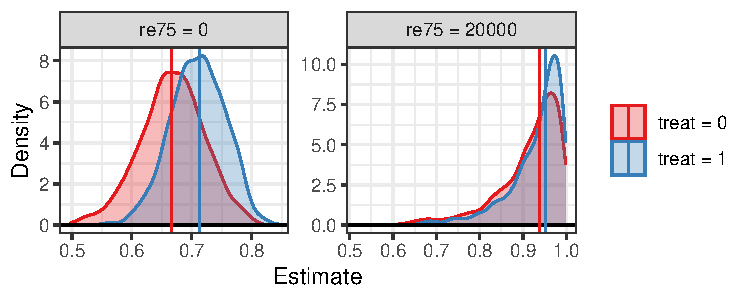
\includegraphics{figures/plot3-1} \end{center}

One can see again how a delta method or Normal approximation may have yielded uncertainty intervals outside the plausible range of the estimate without applying knowledge of the correct transformation to use to avoid doing so.

If a continuous variable with many levels is included in the grid of the predictors, something like a dose-response function for a typical unit can be generated. Below, we set \texttt{re75} to vary from 0 to 20000 in steps of 2000.

\begin{verbatim}
est4 <- sim_setx(s,
                 x = list(treat = 0:1,
                          re75 = seq(0, 20000, by = 2000),
                          race = "black"),
                 verbose = FALSE)
\end{verbatim}

When we plot the output, we can see how the predictions varies across the levels of \texttt{re75}:

\begin{verbatim}
plot(est4)
\end{verbatim}

\begin{center}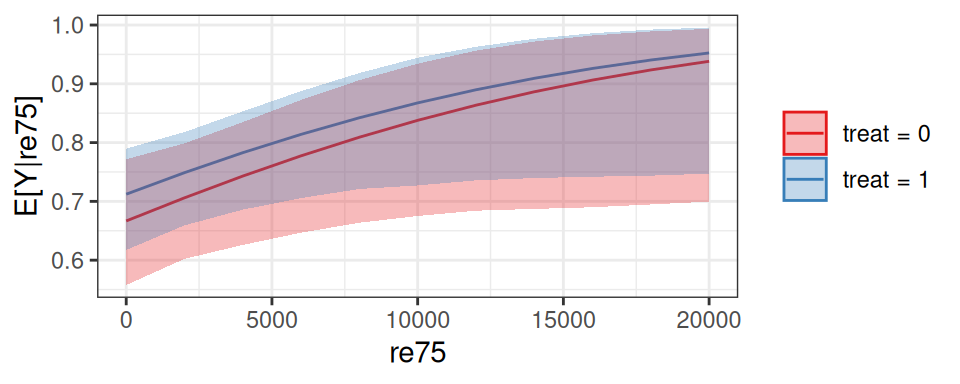
\includegraphics{figures/plot4-1} \end{center}

We will return to display average dose-response functions using \texttt{sim\_adrf()} later.

Finally, we can use \texttt{sim\_setx()} to compute first differences, the contrast between two covariate combinations. We supply one covariate profile to \texttt{x} and another to \texttt{x1}, and \texttt{sim\_setx()} simulates the two predicted values and their difference. Below, we simulate first difference for a treated and control unit who have \texttt{re75} of 0 and typical values of all other covariates:

\begin{verbatim}
est5 <- sim_setx(s,
                 x = list(treat = 0, re75 = 0),
                 x1 = list(treat = 1, re75 = 0),
                 verbose = FALSE)
\end{verbatim}

When we use \texttt{summary()}, we see the estimates for the predicted values and their first difference (``FD''):

\begin{verbatim}
summary(est5)
\end{verbatim}

\begin{verbatim}
#>           Estimate   2.5 %  97.5 %
#> treat = 0   0.7856  0.7039  0.8558
#> treat = 1   0.8213  0.7111  0.8995
#> FD          0.0357 -0.0598  0.1188
\end{verbatim}

It is possible to compute first differences without using \texttt{x1} using \texttt{transform()}, which we describe later.

\hypertarget{sim_ame-average-adjusted-predictions-and-average-marginal-effects}{%
\subsection{\texorpdfstring{\texttt{sim\_ame()}: average adjusted predictions and average marginal effects}{sim\_ame(): average adjusted predictions and average marginal effects}}\label{sim_ame-average-adjusted-predictions-and-average-marginal-effects}}

Using predicted values and effects at representative values is one way to summarize regression models, but another way is to compute average adjusted predictions (AAPs), contrasts of AAPs, and average marginal effects (AMEs). The definitions for these terms may vary and the names for these concepts differ across sources, but here we define AAPs as the average of the predicted values for all units after setting one predictor to a chosen value, and we define AMEs for binary predictors as the contrast of two AAPs and for continuous predictors as the average of instantaneous rate of change in the AAP corresponding to a small change in the predictor from its observed values across all units\footnote{In \CRANpkg{marginaleffects}, AAPs are computed using \texttt{avg\_predictions()}, AMEs for binary variables are computed using \texttt{avg\_comparisons()}, and AMEs for continuous variables are computed using \texttt{avg\_slopes()}. AAPs are sometimes known as average ``counterfactual'' predictions.} (Long and Freese 2014).

The arguments to \texttt{sim\_ame()} are as follows:

\begin{verbatim}
sim_ame(sim = , var = , subset = , by = , contrast = , outcome = ,
        type = , eps = , verbose = , cl = )
\end{verbatim}

\begin{itemize}
\item
  \texttt{sim} -- a \texttt{clarify\_sim} object; the output of a call to \texttt{sim()}.
\item
  \texttt{var} -- the name of focal variable over which to compute the AAPs or AMEs, or a list containing the values for which AAPs should be computed.
\item
  \texttt{subset} -- a logical vector, evaluated in the original dataset used to fit the model, defining a subset of units for which the AAPs or AMEs are to be computed.
\item
  \texttt{by} -- the name of one or more variables for which AAPs should be computed within subgroups. Can be supplied as a character vector of variable names or a one-sided formula.
\item
  \texttt{contrast} -- the name of an effect measure used to contrast AAPs. For continuous outcomes, \texttt{"diff"} requests the difference in means, but others are available for binary outcomes, including \texttt{"rr"} for the risk ratio, \texttt{"or"} for the odds ratio, and \texttt{"nnt"} for the number needed to treat, among others. If not specified, only AAPs will be computed if the variable named in \texttt{var} is categorical or specific values of the focal variable are specified in \texttt{var}. Ignored when the variable named in \texttt{var} is continuous and no specific values are specified because the AME is the only quantity computed. When \texttt{var} names a multi-category categorical variable, \texttt{contrast} cannot be used; see the section describing \texttt{transform()} for computing contrasts with them.
\item
  \texttt{outcome} -- a string containing the name of the outcome of interest when a multivariate (multiple outcome) model is supplied to \texttt{sim()} or the outcome category of interest when a multinomial model is supplied to \texttt{sim()}. For univariate (single outcome) and binary outcomes, this is ignored.
\item
  \texttt{type} -- a string containing the type of predicted value to return. In most cases, this can be left unspecified to request predictions on the scale of the outcome (e.g., probabilities for binary outcomes).
\item
  \texttt{eps} -- the value by which the observed values of the variable named in \texttt{var} are changed when it is continuous to compute the AME. This usually does not need to be specified.
\item
  \texttt{verbose} -- whether to display a progress bar.
\item
  \texttt{cl} -- an argument that controls parallel processing, which can be the number of cores to use or a cluster object resulting from \texttt{parallel::makeCluster()}.
\end{itemize}

Here, we will use \texttt{sim\_ame()} to compute the AME of \texttt{treat} just among those who were treated (in causal inference, this is known as the average treatment effect in the treated, or ATT (Greifer and Stuart 2023)). We will request our estimate to be on the risk ratio scale.

\begin{verbatim}
est6 <- sim_ame(s,
                var = "treat",
                subset = treat == 1,
                contrast = "rr",
                verbose = FALSE)
\end{verbatim}

We can use \texttt{summary()} to display the estimates and their uncertainty intervals. Here, we will also use \texttt{null} to include a test for the null hypothesis that the risk ratio is equal to 1.

\begin{verbatim}
summary(est6, null = c(`RR` = 1))
\end{verbatim}

\begin{verbatim}
#>         Estimate 2.5 % 97.5 % P-value
#> E[Y(0)]    0.687 0.608  0.760       .
#> E[Y(1)]    0.755 0.685  0.809       .
#> RR         1.100 0.949  1.255    0.21
\end{verbatim}

Here we see the estimates for the AAPs, \texttt{E{[}Y(0){]}} for the expected value of the outcome setting \texttt{treat} to 0 and \texttt{E{[}Y(1){]}} for the expected value of the outcome setting \texttt{treat} to 1, and the risk ratio \texttt{RR}. The p-value on the test for the risk ratio aligns with the uncertainty interval containing 1.

If we instead wanted the risk difference or odds ratio, we would not have to re-compute the AAPs. Instead, we can use \texttt{transform()} to compute a new derived quantity from the computed AAPs. The section on \texttt{transform()} demonstrates this.

We can compute the AME for a continuous predictor. Here, we will consider \texttt{age} (just for demonstration; this analysis does not have a valid interpretation).

\begin{verbatim}
est7 <- sim_ame(s,
                var = "age",
                verbose = FALSE)
\end{verbatim}

We can use \texttt{summary()} to display the AME estimate and its uncertainty interval.

\begin{verbatim}
summary(est7)
\end{verbatim}

\begin{verbatim}
#>              Estimate    2.5 %   97.5 %
#> E[dY/d(age)] -0.00605 -0.00940 -0.00259
\end{verbatim}

The AME is named \texttt{E{[}dY/d(age){]}}, which signifies that a derivative has been computed (more precisely, the average of the unit-specific derivatives). This estimate can be interpreted like a slope in a linear regression model, but as a single summary of the effect of a predictor it is often too coarse to capture nonlinear relationships. The section below explains how to compute average dose-response functions for continuous predictors, which provide a more complete picture of their effects on an outcome.

Below, we will examine effect modification of the ATT by the predictor \texttt{married} using the \texttt{by} argument to estimate AAPs and their ratio within levels of \texttt{married}:

\begin{verbatim}
est6b <- sim_ame(s,
                 var = "treat",
                 subset = treat == 1,
                 by = ~married,
                 contrast = "rr",
                 verbose = FALSE)

summary(est6b)
\end{verbatim}

\begin{verbatim}
#>           Estimate 2.5 % 97.5 %
#> E[Y(0)|0]    0.691 0.612  0.768
#> E[Y(1)|0]    0.733 0.655  0.796
#> RR[0]        1.061 0.909  1.234
#> E[Y(0)|1]    0.668 0.556  0.769
#> E[Y(1)|1]    0.848 0.676  0.940
#> RR[1]        1.270 0.948  1.583
\end{verbatim}

The presence of effect modification can be tested by testing the contrast between the effects computed within each level of the \texttt{by} variable; this demonstrated in the section on \texttt{transform()} below.

\hypertarget{sim_adrf-average-dose-response-functions}{%
\subsection{\texorpdfstring{\texttt{sim\_adrf()}: average dose-response functions}{sim\_adrf(): average dose-response functions}}\label{sim_adrf-average-dose-response-functions}}

A dose-response function for an individual is the relationship between the set value of a continuous focal predictor and the expected outcome. The average dose-response function (ADRF) is the average of the dose-response functions across all units. Essentially, it is a function that relates the value of the predictor to the corresponding AAP of the outcome, the average value of the outcome were all units to be set to that level of the predictor. ADRFs can be used to provide additional detail about the effect of a continuous predictor beyond a single AME.

A related quantity is the average marginal effect function (AMEF), which describes the relationship between a continuous focal predictor and the AME at that level of the predictor. That is, rather than describing how the outcome changes as a function of the predictor, it describes how the \emph{effect} of the predictor on the outcome changes as a function of the predictor. It is essentially the derivative of the ADRF and can be used to identify at which points along the ADRF the predictor has an effect.

The ADRF and AMEF can be computed using \texttt{sim\_adrf()}. The arguments are below:

\begin{verbatim}
sim_adrf(sim = , var = , subset = , by = , contrast = , at = ,
         n = , outcome = , type = , eps = , verbose = , cl = )
\end{verbatim}

\begin{itemize}
\item
  \texttt{sim} -- a \texttt{clarify\_sim} object; the output of a call to \texttt{sim()}.
\item
  \texttt{var} -- the name of focal variable over which to compute the ADRF or AMEF.
\item
  \texttt{subset} -- a logical vector, evaluated in the original dataset used to fit the model, defining a subset of units for which the ARDF or AMEF is to be computed.
\item
  \texttt{by} -- the name of one or more variables for which the ADRF or AMEF should be computed within subgroups. Can be supplied as a character vector of variable names or a one-sided formula.
\item
  \texttt{contrast} -- either \texttt{"adrf"} or \texttt{"amef"} to request the ADRF or AMEF, respectively. The default is to compute the ADRF.
\item
  \texttt{at} -- the values of the focal predictor at which to compute the ADRF or AMEF. This should be a vector of values that the focal predictor can take on. If unspecified, a vector of \texttt{n} (see below) equally-spaced values from the minimum to the maximum value of the predictor will be used. This should typically be used only if quantities are desired over a subset of the values of the focal predictor.
\item
  \texttt{n} -- if \texttt{at} is unspecified, the number of points along the range of the focal predictor at which to compute the ADRF or AMEF. More yields smoother functions, but will take longer and require more memory. The default is 21.
\item
  \texttt{outcome} -- a string containing the name of the outcome of interest when a multivariate (multiple outcome) model is supplied to \texttt{sim()} or the outcome category of interest when a multinomial model is supplied to \texttt{sim()}. For univariate (single outcome) and binary outcomes, this is ignored.
\item
  \texttt{type} -- a string containing the type of predicted value to return. In most cases, this can be left unspecified to request predictions on the scale of the outcome.
\item
  \texttt{eps} -- the value by which the observed values of the variable named in \texttt{var} are changed when it is continuous to compute the AMEF. This usually does not need to be specified.
\item
  \texttt{verbose} -- whether to display a progress bar.
\item
  \texttt{cl} -- an argument that controls parallel processing, which can be the number of cores to use or a cluster object resulting from \texttt{parallel::makeCluster()}.
\end{itemize}

Here, we will consider \texttt{age} (just for demonstration; this analysis does not have a valid interpretation) and compute the ADRF and AMEF of \texttt{age} on the outcome. We will only examine ages between 18 and 50, even though the range of \texttt{age} goes slightly beyond these values. First, we will compute the ADRF of \texttt{age}, which examines how the outcome would vary on average if one set all unit's value of \texttt{age} to each value between 18 and 50 (here we only use even ages to speed up computation).

\begin{verbatim}
age_seq <- seq(18, 50, by = 2)

est8 <- sim_adrf(s,
                 var = "age",
                 contrast = "adrf",
                 at = age_seq,
                 verbose = FALSE)
\end{verbatim}

We can plot the ADRF using \texttt{plot()}.

\begin{verbatim}
plot(est8)
\end{verbatim}

\begin{center}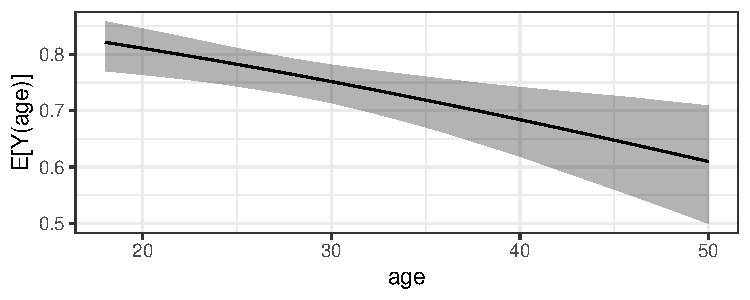
\includegraphics{figures/plot8-1} \end{center}

From the plot, we can see that as \texttt{age} increases, the expected outcome decreases.

We can also examine the AAPs at the requested ages using \texttt{summary()}, which will display all the estimated AAPs by default, so we will request just the first 4 (\texttt{age}s 18 to 24):

\begin{verbatim}
summary(est8, parm = 1:4)
\end{verbatim}

\begin{verbatim}
#>          Estimate 2.5 % 97.5 %
#> E[Y(18)]    0.821 0.771  0.858
#> E[Y(20)]    0.811 0.764  0.845
#> E[Y(22)]    0.800 0.757  0.832
#> E[Y(24)]    0.788 0.749  0.817
\end{verbatim}

Next we will compute the AMEF, the effect of \texttt{age} at each level of \texttt{age}.

\begin{verbatim}
est9 <- sim_adrf(s,
                 var = "age",
                 contrast = "amef",
                 at = age_seq,
                 verbose = FALSE)
\end{verbatim}

We can plot the AMEF using \texttt{plot()}:

\begin{verbatim}
plot(est9)
\end{verbatim}

\begin{center}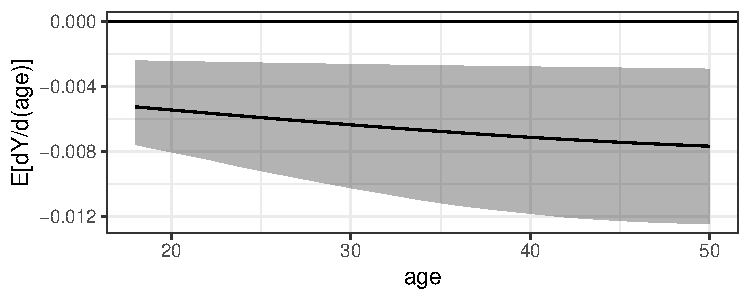
\includegraphics{figures/plot9-1} \end{center}

From the plot, we can see the AME of \texttt{age} decreases slightly but is mostly constant across values of \texttt{age}, and the uncertainty intervals for the AMEs consistently exclude 0.

\hypertarget{transforming-and-combining-estimates}{%
\section{Transforming and Combining Estimates}\label{transforming-and-combining-estimates}}

Often, our quantities of interest are not just the outputs of the functions above, but comparisons between them. For example, to test for moderation of a treatment effect, we may want to compare AMEs in multiple groups defined by the moderator. Or, it might be that we are interested in an effect described using a different effect measure than the one originally produced; for example, we may decide we want the risk difference AME after computing the risk ratio AME. The functions \texttt{transform()} and \texttt{cbind()} allow users to transform quantities in a single \texttt{clarify\_est} object and combine two \texttt{clarify\_est} objects. These are essential for computing quantities that themselves are derived from the derived quantities computed by the \texttt{sim\_*()} functions.

\hypertarget{transform}{%
\subsection{\texorpdfstring{\texttt{transform()}}{transform()}}\label{transform}}

\texttt{transform()} is a generic function in R that is typically used to create a new variable in a data frame that is a function of other columns. For example, to compute the binary outcome we used in our model, we could have run the following\footnote{Users familiar with the \texttt{tidyverse} will note the similarities between \texttt{transform()} and \texttt{dplyr::mutate()}; only \texttt{transform()} can be used with \texttt{clarify\_est} objects.}:

\begin{verbatim}
lalonde <- transform(lalonde,
                     re78_0 = ifelse(re78 == 0, 1, 0))
\end{verbatim}

Similarly, to compute a derived or transformed quantity from a \texttt{clarify\_est} object, we can use \texttt{transform()}. Here, we will compute the risk difference AME of \texttt{treat}; previously, we used \texttt{sim\_ame()} to compute the AAPs and the risk ratio.

\begin{verbatim}
est6 <- transform(est6,
                  RD = `E[Y(1)]` - `E[Y(0)]`)
\end{verbatim}

Note that we used tics (\texttt{\textasciigrave{}}) around the names of the AAPs; this is necessary when they contain special characters like parentheses or brackets. An alternative is to use the shortcut names \texttt{.b\#}, where \texttt{\#} is replaced with a number (e.g., as \texttt{.b1}, \texttt{.b2}, etc.) corresponding to the index of the quantity referenced. For example, because \texttt{E{[}Y(1){]}}and\texttt{E{[}Y(0){]}} are the second and first computed quantities, respectively, the above code could be replaced with

\begin{verbatim}
est6 <- transform(est6,
                  RD = .b2 - .b1)
\end{verbatim}

which will yield identical results\footnote{Note that if a quantity is named \texttt{.b\#}, e.g., \texttt{.b1}, it can only be referred to using the positional shortcut and not its named. That is, the positional shortcut takes precedence over the names of the quantities.}.

When we run \texttt{summary()} on the output, the new quantity, which we named ``RD'', will be displayed along with the other estimates. We will also set a null value for this quantity.

\begin{verbatim}
summary(est6, null = c(`RR` = 1, `RD` = 0))
\end{verbatim}

\begin{verbatim}
#>         Estimate   2.5 %  97.5 % P-value
#> E[Y(0)]   0.6866  0.6081  0.7596       .
#> E[Y(1)]   0.7551  0.6850  0.8088       .
#> RR        1.0998  0.9485  1.2554    0.21
#> RD        0.0685 -0.0382  0.1580    0.21
\end{verbatim}

As mentioned previously, one benefit of using simulation-based inference with p-values computed from inverting the confidence intervals is that the p-values for testing the same hypothesis with the risk difference and risk ratio (and any other effect measure for comparing a pair of values) will always exactly align, thereby ensuring inference does not depend on the effect measure used. In contrast, Wald-type inference (based on either the simulation-derived or delta method standard error) is not invariant to transformations of the quantity of interest.

The same value would be computed if we were to have called \texttt{sim\_ame()} on the same \texttt{clarify\_sim} object and requested the risk difference using \texttt{contrast\ =\ "diff"}; using \texttt{transform()} saves time because the AAPs are already computed and stored in the \texttt{clarify\_est} object.

We can use \texttt{transform()} along with the \texttt{by} variable in \texttt{sim\_ame()} to compute the contrast between quantities computed within each subgroup of \texttt{married}. Previously we used \texttt{by} to compute the risk ratio ATT within levels of \texttt{married}; here we will compute the ratio of these risk ratios to assess the presence of effect modification.

\begin{verbatim}
est6b |>
  transform(`RR[1]/RR[0]` = `RR[1]` / `RR[0]`) |>
  summary(parm = c("RR[0]", "RR[1]", "RR[1]/RR[0]"),
          null = 1)
\end{verbatim}

\begin{verbatim}
#>             Estimate 2.5 % 97.5 % P-value  
#> RR[0]          1.061 0.909  1.234   0.434  
#> RR[1]          1.270 0.948  1.583   0.094 .
#> RR[1]/RR[0]    1.196 0.908  1.516   0.174  
#> ---
#> Signif. codes:  0 '***' 0.001 '**' 0.01 '*' 0.05 '.' 0.1 ' ' 1
\end{verbatim}

\texttt{RR{[}1{]}/RR{[}0{]}} contains the ratio of the risk ratios for \texttt{married\ =\ 1} and \texttt{married\ =\ 0}. Here we also include a test for whether each of the risk ratios and their ratio differ from 1, which is equivalent to testing whether the risk ratios differ across levels of \texttt{married}.

\hypertarget{cbind}{%
\subsection{\texorpdfstring{\texttt{cbind()}}{cbind()}}\label{cbind}}

\texttt{cbind()} is another generic R function that is typically used to combine two or more datasets columnwise (i.e., to widen a dataset). In \CRANpkg{clarify}, \texttt{cbind()} can be used to combine two \texttt{clarify\_est} objects so that the estimates can be examined jointly and so that it is possible to compare them directly. For example, if we were to compute AMEs in two subgroups using \texttt{subset} and wanted to compare them, we would call \texttt{sim\_ame()} twice, one for each subset (though in practice it is more effective to use \texttt{by}; this is just for illustration), as demonstrated below:

\begin{verbatim}
# AME of treat with race = "black"
est10b <- sim_ame(s, var = "treat", subset = race == "black",
                  contrast = "diff", verbose = FALSE)
summary(est10b)
\end{verbatim}

\begin{verbatim}
#>         Estimate   2.5 %  97.5 %
#> E[Y(0)]   0.6677  0.5813  0.7529
#> E[Y(1)]   0.7439  0.6661  0.8016
#> Diff      0.0762 -0.0359  0.1700
\end{verbatim}

\begin{verbatim}
# AME of treat with race = "hispan"
est10h <- sim_ame(s, var = "treat", subset = race == "hispan",
                  contrast = "diff", verbose = FALSE)
summary(est10h)
\end{verbatim}

\begin{verbatim}
#>         Estimate   2.5 %  97.5 %
#> E[Y(0)]   0.8266  0.7146  0.8990
#> E[Y(1)]   0.8971  0.7888  0.9527
#> Diff      0.0704 -0.0223  0.1387
\end{verbatim}

Here, we computed the risk difference for the subgroups \texttt{race\ =\ "black"} and \texttt{race\ =\ "hispan"}. If we wanted to compare the risk differences, we could combine them and compute a new quantity equal to their difference. We will do that below.

First, we need to rename the quantities in each object so they do not overlap; we can do so using \texttt{names()}, which has a special method for \texttt{clarify\_est} objects.

\begin{verbatim}
names(est10b) <- paste(names(est10b), "b", sep = "_")
names(est10h) <- paste(names(est10h), "h", sep = "_")
\end{verbatim}

Next, we use \texttt{cbind()} to bind the objects together.

\begin{verbatim}
est10 <- cbind(est10b, est10h)
summary(est10)
\end{verbatim}

\begin{verbatim}
#>           Estimate   2.5 %  97.5 %
#> E[Y(0)]_b   0.6677  0.5813  0.7529
#> E[Y(1)]_b   0.7439  0.6661  0.8016
#> Diff_b      0.0762 -0.0359  0.1700
#> E[Y(0)]_h   0.8266  0.7146  0.8990
#> E[Y(1)]_h   0.8971  0.7888  0.9527
#> Diff_h      0.0704 -0.0223  0.1387
\end{verbatim}

Finally, we can use \texttt{transform()} to compute the difference between the risk differences:

\begin{verbatim}
est10 <- transform(est10,
                   `Dh - Db` = Diff_h - Diff_b)
summary(est10, parm = "Dh - Db")
\end{verbatim}

\begin{verbatim}
#>         Estimate    2.5 %   97.5 %
#> Dh - Db -0.00575 -0.06833  0.04103
\end{verbatim}

Importantly, \texttt{cbind()} can only be used to join together \texttt{clarify\_est} objects computed using the same simulated coefficients (i.e., resulting from the same call to \texttt{sim()}). This preserves the covariance among the estimated quantities, which is critical for maintaining valid inference. That is, \texttt{sim()} should only be called once per model, and all derived quantities should be computed using its output.

\hypertarget{using-with-multiply-imputed-data}{%
\section{\texorpdfstring{Using \pkg{clarify} with Multiply Imputed Data}{Using  with Multiply Imputed Data}}\label{using-with-multiply-imputed-data}}

Multiple imputation is a popular method of estimating quantities of interest in the presence of missing data and involves creating multiple versions of the original dataset each with the missing values imputed with estimates from an imputation model. Simulation-based inference in multiply imputed data is relatively straightforward. Simulated coefficients are drawn from the model estimated in each imputed dataset separately, and then the simulated coefficients are pooled into a single set of simulated coefficients. In Bayesian terms, this would be considered ``mixing draws'' and is the recommended approach for Bayesian analysis with multiply imputed data (Zhou and Reiter 2010).

Using \CRANpkg{clarify} with multiply imputed data is simple. Rather than using \texttt{sim()}, we use the function \texttt{misim()}. \texttt{misim()} functions just like \texttt{sim()} except that it takes in a list of model fits (i.e., containing a model fit to each imputed dataset) or an object containing such a list (e.g., a \texttt{mira} object from \texttt{mice::with()} or a \texttt{mimira} object from \texttt{MatchThem::with()}). \texttt{misim()} simulates coefficient distributions within each imputed dataset and then appends them together to a form a single combined set of coefficient draws.

\texttt{sim\_apply()} and its wrappers accept the output of \texttt{misim()} and compute the desired quantity using each set of coefficients. When these functions rely on using a dataset (e.g., \texttt{sim\_ame()}, which averages predicted outcomes across all units in the dataset used to fit the model), they automatically know to associate a given coefficient draw with the imputed dataset that was used to fit the model that produced that draw. In user-written functions supplied to the \texttt{FUN} argument of \texttt{sim\_apply()}, it is important to correctly extract the dataset from the model fit. This is demonstrated below.

The final estimates of the quantity of interest is computed as the mean of the estimates computed in each imputed dataset (i.e., using the original coefficients, not the simulated ones), which is the same quantity that would be computed using standard pooling rules. This is not always valid for noncollapsible estimates, like ratios, and so care should be taken to ensure the mean of the resulting estimates has a valid interpretation (this is related to the transformation-induced bias described by Rainey (2017)).

The arguments to \texttt{misim()} are as follows:

\begin{verbatim}
misim(fitlist = , n = , vcov = , coefs = , dist = )
\end{verbatim}

\begin{itemize}
\item
  \texttt{fitlist} -- a list of model fits or an accepted object containing them (e.g., a \texttt{mira} object from \texttt{mice::with()})
\item
  \texttt{n} -- the number of simulations to run \emph{for each imputed dataset}. The default is 1000, but fewer can be used because the total number of simulated quantities will be \texttt{m\ *\ n}, where \texttt{m} is the number of imputed datasets.
\item
  \texttt{vcov}, \texttt{coefs}, \texttt{dist} -- the same as with \texttt{sim()}, except that a list of such arguments can be supplied to be applied to each imputed dataset.
\end{itemize}

Below we illustrate using \texttt{misim()} and \texttt{sim\_apply()} with multiply imputed data. We will use the \texttt{africa} dataset from the \CRANpkg{Amelia} package.

\begin{verbatim}
library(Amelia)
data("africa", package = "Amelia")

# Multiple imputation
a.out <- amelia(x = africa, m = 10, cs = "country",
                ts = "year", logs = "gdp_pc", p2s = 0)

# Fit model to each dataset
model.list <- with(a.out, lm(gdp_pc ~ infl * trade))

# Simulate coefficients, 100 draws per imputation
si <- misim(model.list, n = 100)

si
\end{verbatim}

\begin{verbatim}
#> A `clarify_misim` object
#>  - 4 coefficients, 10 imputations with 100 simulated values each
#>  - sampled distributions: multivariate t(116)
\end{verbatim}

The function we will be applying to each imputed dataset will be one that computes the AME of \texttt{infl}. (We will run the same analysis afterward using \texttt{sim\_ame()}.)

\begin{verbatim}
sim_fun <- function(fit) {
  #Extract the original dataset using get_predictors()
  X <- insight::get_predictors(fit)
  
  p0 <- predict(fit)
  
  #Predictions after perturbing infl slightly
  p1 <- predict(fit, newdata = transform(X, infl = infl + 1e-5))
  
 c(AME = mean((p1 - p0) / 1e-5))
}

est_mi <- sim_apply(si, FUN = sim_fun, verbose = FALSE)

summary(est_mi)
\end{verbatim}

\begin{verbatim}
#>     Estimate 2.5 % 97.5 %
#> AME    -5.75 -8.82  -2.26
\end{verbatim}

Note that \texttt{sim\_apply()} ``knows'' which imputation produced each set of simulated coefficients, so using \texttt{insight::get\_predictors()} on the \texttt{fit} supplied to \texttt{sim\_fun()} will use the right dataset. Care should be taken when analyses restrict each imputed dataset in a different way (e.g.~when matching with a caliper in each one), as the resulting imputations may not refer to a specific target population and mixing the draws may be invalid.

Below, we can use \texttt{sim\_ame()}:

\begin{verbatim}
est_mi2 <- sim_ame(si, var = "infl", verbose = FALSE)

summary(est_mi2)
\end{verbatim}

\begin{verbatim}
#>               Estimate 2.5 % 97.5 %
#> E[dY/d(infl)]    -5.75 -8.82  -2.26
\end{verbatim}

We get the same results, as expected.

Note that \texttt{misim()} is compatible with model fit objects from \CRANpkg{mice}, \CRANpkg{Amelia}, \CRANpkg{MatchThem}, and any other package that produces a list of model fit objects with each corresponding to the output of a model fit to an imputed dataset.

\hypertarget{comparison-to-other-packages}{%
\section{Comparison to Other Packages}\label{comparison-to-other-packages}}

Several packages offer methods for computing interpretable quantities form regression models, including \CRANpkg{emmeans} (Lenth 2024), \pkg{margins} (Leeper 2021), \CRANpkg{modelbased} (Makowski et al. 2020), and \CRANpkg{marginaleffects} (Arel-Bundock, Greifer, and Heiss Forthcoming). Many of the quantities computed by these packages can also be computed by \CRANpkg{clarify}, the primary difference being that \CRANpkg{clarify} uses simulation-based inference rather than delta method-based inference.

\CRANpkg{marginaleffects} offers the most similar functionality to \CRANpkg{clarify}, and \CRANpkg{clarify} depends on functionality provided by \CRANpkg{marginaleffects} to accommodate a wide variety of regression models. \CRANpkg{marginaleffects} also offers simulation-based inference using \texttt{marginaleffects::inferences()} and support for arbitrary user-specified post-estimation functions using \texttt{marginaleffects::hypotheses()}. However, \CRANpkg{clarify} and \texttt{marignalefefcts} differ in several ways. The largest difference is that \CRANpkg{clarify} supports iterative building of more and more complex hypotheses through the \texttt{transform()} method, which quickly computes new quantities and transformation from the existing computed quantities, whereas \CRANpkg{marginaleffects} only supports a single transformation and, as of version 0.20.0, cannot use simulation-based inference for these quantities.

Because of \CRANpkg{clarify}'s focus on simulation, it provides functionality directly aimed at improving simulation-based inference, including plots to view the distributions of simulated values and support for parallel processing. \CRANpkg{clarify} also provides support for simulation-based inference of multiply imputed data, which does not require any special pooling rules.

There are areas and cases where \CRANpkg{marginaleffects} may be the better choice than \CRANpkg{clarify} or where the differences between the packages are of little consequence. \CRANpkg{marginaleffects} focuses on providing a complete framework for post-estimation using model predictions, whereas \CRANpkg{clarify} is primarily focused on supporting user-defined functions, with commonly used estimators offered as a convenience. In cases where the delta method is an acceptable approximation (e.g., for quantities computed from linear models or other quantities known to be approximately Normally distributed in finite samples), using the delta method through \CRANpkg{marginaleffects} will be much faster, more accurate, and more replicable than the simulation-based inference \CRANpkg{clarify} provides. For the quantities easily computed by \CRANpkg{marginaleffects} that support simulation-based inference through \texttt{marginaleffects::inferences()}, using \CRANpkg{marginaleffects} can provide a more familiar and flexible syntax than \CRANpkg{clarify} might offer. Ultimately, the user should use the package that supports their desired syntax and mode of inference.

\hypertarget{conclusion}{%
\section{Conclusion}\label{conclusion}}

\CRANpkg{clarify} provides functionality to facilitate simulation-based inference of deriving quantities from regression models. This framework provides an alternative to the delta method that can yield confidence intervals with closer to nominal coverage for some quantities of interest. While we do not claim simulation-based inference should be universally preferred over delta method-based inference, there are cases in which it can retain some advantageous properties, and we hope the availability of these methods in \CRANpkg{clarify} encourages additional research on when those properties can be realized and facilitates empirical work that takes advantages of these properties.

\hypertarget{references}{%
\section*{References}\label{references}}
\addcontentsline{toc}{section}{References}

\hypertarget{refs}{}
\begin{CSLReferences}{1}{0}
\leavevmode\vadjust pre{\hypertarget{ref-marginaleffectsforthcoming}{}}%
Arel-Bundock, Vincent, Noah Greifer, and Andrew Heiss. Forthcoming. {``How to Intepret Statistical Models Using {marginaleffects} in {R} and {Python}.''} \emph{Journal of Statistical Software}, Forthcoming.

\leavevmode\vadjust pre{\hypertarget{ref-dehejiaCausalEffectsNonexperimental1999}{}}%
Dehejia, Rajeev H., and Sadek Wahba. 1999. {``Causal Effects in Nonexperimental Studies: Reevaluating the Evaluation of Training Programs.''} \emph{Journal of the American Statistical Association} 94 (448): 1053--62. \url{https://doi.org/10.1080/01621459.1999.10473858}.

\leavevmode\vadjust pre{\hypertarget{ref-efronBootstrapMethodsStandard1986}{}}%
Efron, B., and R. Tibshirani. 1986. {``Bootstrap Methods for Standard Errors, Confidence Intervals, and Other Measures of Statistical Accuracy.''} \emph{Statistical Science} 1 (1): 54--75. \url{https://www.jstor.org/stable/2245500}.

\leavevmode\vadjust pre{\hypertarget{ref-greiferChoosingCausalEstimand2023}{}}%
Greifer, Noah, and Elizabeth A. Stuart. 2023. {``Choosing the Causal Estimand for Propensity Score Analysis of Observational Studies.''} \url{https://doi.org/10.48550/arXiv.2106.10577}.

\leavevmode\vadjust pre{\hypertarget{ref-herronPostestimationUncertaintyLimited1999}{}}%
Herron, Michael C. 1999. {``Postestimation Uncertainty in Limited Dependent Variable Models.''} \emph{Political Analysis} 8 (1): 83--98. \url{https://doi.org/10.1093/oxfordjournals.pan.a029806}.

\leavevmode\vadjust pre{\hypertarget{ref-JSSv042i08}{}}%
Ho, Daniel E., Kosuke Imai, Gary King, and Elizabeth A. Stuart. 2011. {``MatchIt: Nonparametric Preprocessing for Parametric Causal Inference.''} \emph{Journal of Statistical Software, Articles} 42 (8): 128. \url{https://doi.org/10.18637/jss.v042.i08}.

\leavevmode\vadjust pre{\hypertarget{ref-holeComparisonApproachesEstimating2007}{}}%
Hole, Arne Risa. 2007. {``A Comparison of Approaches to Estimating Confidence Intervals for Willingness to Pay Measures.''} \emph{Health Economics} 16 (8): 827--40. \url{https://doi.org/10.1002/hec.1197}.

\leavevmode\vadjust pre{\hypertarget{ref-imaiCommonFrameworkStatistical2008a}{}}%
Imai, Kosuke, Gary King, and Olivia Lau. 2008. {``Toward a Common Framework for Statistical Analysis and Development.''} \emph{Journal of Computational and Graphical Statistics} 17 (4): 892--913. \url{https://doi.org/10.1198/106186008X384898}.

\leavevmode\vadjust pre{\hypertarget{ref-kingMakingMostStatistical2000}{}}%
King, Gary, Michael Tomz, and Jason Wittenberg. 2000. {``Making the Most of Statistical Analyses: Improving Interpretation and Presentation.''} \emph{American Journal of Political Science} 44 (2): 347--61. \url{https://doi.org/10.2307/2669316}.

\leavevmode\vadjust pre{\hypertarget{ref-krinsky1986}{}}%
Krinsky, Itzhak, and A. Leslie Robb. 1986. {``On Approximating the Statistical Properties of Elasticities.''} \emph{The Review of Economics and Statistics} 68 (4): 715. \url{https://doi.org/10.2307/1924536}.

\leavevmode\vadjust pre{\hypertarget{ref-margins2021}{}}%
Leeper, Thomas J. 2021. \emph{Margins: Marginal Effects for Model Objects}.

\leavevmode\vadjust pre{\hypertarget{ref-emmeans2024}{}}%
Lenth, Russell V. 2024. \emph{Emmeans: Estimated Marginal Means, Aka Least-Squares Means}. \url{https://CRAN.R-project.org/package=emmeans}.

\leavevmode\vadjust pre{\hypertarget{ref-longRegressionModelsCategorical2014}{}}%
Long, J. Scott, and Jeremy Freese. 2014. \emph{Regression Models for Categorical Dependent Variables Using Stata}. Third edition. College Station, Texas: Stata Press Publication, StataCorp LP.

\leavevmode\vadjust pre{\hypertarget{ref-mackinnonConfidenceLimitsIndirect2004}{}}%
MacKinnon, David P., Chondra M. Lockwood, and Jason Williams. 2004. {``Confidence Limits for the Indirect Effect: Distribution of the Product and Resampling Methods.''} \emph{Multivariate Behavioral Research} 39 (1): 99--128. \url{https://doi.org/10.1207/s15327906mbr3901_4}.

\leavevmode\vadjust pre{\hypertarget{ref-modelbased2020}{}}%
Makowski, Dominique, Mattan S. Ben-Shachar, Indrajeet Patil, and Daniel Lüdecke. 2020. {``Estimation of Model-Based Predictions, Contrasts and Means.''} \emph{CRAN}. \url{https://github.com/easystats/modelbased}.

\leavevmode\vadjust pre{\hypertarget{ref-preacherAdvantagesMonteCarlo2012}{}}%
Preacher, Kristopher J., and James P. Selig. 2012. {``Advantages of Monte Carlo Confidence Intervals for Indirect Effects.''} \emph{Communication Methods and Measures} 6 (2): 77--98. \url{https://doi.org/10.1080/19312458.2012.679848}.

\leavevmode\vadjust pre{\hypertarget{ref-rainey2017}{}}%
Rainey, Carlisle. 2017. {``Transformation-Induced Bias: Unbiased Coefficients Do Not Imply Unbiased Quantities of Interest.''} \emph{Political Analysis} 25 (3): 402--9. \url{https://doi.org/10.1017/pan.2017.11}.

\leavevmode\vadjust pre{\hypertarget{ref-raineyCarefulConsiderationCLARIFY2023}{}}%
---------. 2023. {``A Careful Consideration of {CLARIFY}: Simulation-Induced Bias in Point Estimates of Quantities of Interest.''} \emph{Political Science Research and Methods}, April, 1--10. \url{https://doi.org/10.1017/psrm.2023.8}.

\leavevmode\vadjust pre{\hypertarget{ref-thulinModernStatisticsWrangling2021}{}}%
Thulin, Måns. 2021. \emph{Modern Statistics with r: From Wrangling and Exploring Data to Inference and Predictive Modelling}. Uppsala, Sweden: Eos Chasma Press.

\leavevmode\vadjust pre{\hypertarget{ref-tofighiMonteCarloConfidence2016}{}}%
Tofighi, Davood, and David P. MacKinnon. 2016. {``Monte Carlo Confidence Intervals for Complex Functions of Indirect Effects.''} \emph{Structural Equation Modeling: A Multidisciplinary Journal} 23 (2): 194205. \url{https://doi.org/10.1080/10705511.2015.1057284}.

\leavevmode\vadjust pre{\hypertarget{ref-tomzClarifySoftwareInterpreting2003}{}}%
Tomz, Michael, Jason Wittenberg, and Gary King. 2003. {``Clarify: Software for Interpreting and Presenting Statistical Results.''} \emph{Journal of Statistical Software} 8 (January): 1--30. \url{https://doi.org/10.18637/jss.v008.i01}.

\leavevmode\vadjust pre{\hypertarget{ref-zelnerUsingSimulationInterpret2009}{}}%
Zelner, Bennet A. 2009. {``Using simulation to interpret results from logit, probit, and other nonlinear models.''} \emph{Strategic Management Journal} 30 (12): 1335--48. \url{https://doi.org/10.1002/smj.783}.

\leavevmode\vadjust pre{\hypertarget{ref-zhouNoteBayesianInference2010}{}}%
Zhou, Xiang, and Jerome P. Reiter. 2010. {``A Note on Bayesian Inference After Multiple Imputation.''} \emph{The American Statistician} 64 (2): 159--63. \url{https://doi.org/10.1198/tast.2010.09109}.

\end{CSLReferences}


\address{%
Noah Greifer\\
Harvard University\\%
Institute for Quantitative Social Science\\ Cambridge, MA\\
%
ngreifer.github.io\\%
\textit{ORCiD: \href{https://orcid.org/0000-0003-3067-7154}{0000-0003-3067-7154}}\\%
\href{mailto:ngreifer@iq.harvard.edu}{\nolinkurl{ngreifer@iq.harvard.edu}}%
}

\address{%
Steven Worthington\\
Harvard University\\%
Institute for Quantitative Social Science\\ Cambridge, MA\\
%
%
\textit{ORCiD: \href{https://orcid.org/0000-0001-9550-5797}{0000-0001-9550-5797}}\\%
\href{mailto:sworthington@iq.harvard.edu}{\nolinkurl{sworthington@iq.harvard.edu}}%
}

\address{%
Stefano Iacus\\
Harvard University\\%
Institute for Quantitative Social Science\\ Cambridge, MA\\
%
%
\textit{ORCiD: \href{https://orcid.org/0000-0002-4884-0047}{0000-0002-4884-0047}}\\%
\href{mailto:siacus@iq.harvard.edu}{\nolinkurl{siacus@iq.harvard.edu}}%
}

\address{%
Gary King\\
Harvard University\\%
Institute for Quantitative Social Science\\ Cambridge, MA\\
%
%
\textit{ORCiD: \href{https://orcid.org/0000-0002-5327-7631}{0000-0002-5327-7631}}\\%
\href{mailto:king@harvard.edu}{\nolinkurl{king@harvard.edu}}%
}
